\subsection{Progettazione di dettaglio e codifica}
Questa fase comincia in seguito a quella precedente e termina con la \textit{Revisione di Qualifica}, ovvero dal 08/03/2020 al 02/04/2020. Di seguito vengono riportate tutte le attività.

\begin{itemize}
	\item \textbf{Incremento e verifica dei documenti}: verrà realizzato un documento contenente tutte le caratteristiche del prodotto e il cosiddetto \textit{Manuale utente}. Inoltre, in caso di necessità, alcuni documenti verranno aggiornati;
	\item \textbf{Incremento e verifica delle attività}: viene ampliato lo studio delle tecnologie mancanti, necessarie per lo sviluppo del prodotto; 
	\item \textbf{\glo{Product Baseline}}: vengono realizzati i \textit{diagrammi delle classi}, che consentono di descrivere tipi di entità (con le loro caratteristiche e le eventuali relazioni), e i \textit{diagrammi delle attività}, che permettono di descrivere i vari processi. Inoltre verranno analizzati design patterns esistenti, con il fine di scegliere quello più adatto per il prodotto da creare.
	\item \textbf{\glo{Scrittura del codice e incrementi}}: viene realizzata la codifica, partendo dal \textit{Proof of Concept} già presente. Gli incrementi consistono nell'implementare sempre più casi d'uso, stabiliti nell'\textit{Analisi dei Rischi}, iterando tra progettazione di dettaglio e realizzazione. La priorità sarà nei confronti di quelli obbligatori: in questo modo per ciascun caso d'uso, nell'eventualità di mancato completamento entro il periodo stabilito, è possibile attuare in sicurezza una ripianificazione dell'attività in questione. \\
	
	\begin{itemize}
	\item \textbf{Incremento 1}: il gruppo si prepara alle attività di progettazione di dettaglio e codifica, inoltre verranno incrementanti i documenti per verifica e miglioramento continuo;
	
	\item \textbf{Incremento 2}: viene studiata la libreria D3.js per individuare i parametri configurabili della visualizzazione Scatter Plot Matrix, e successivamente implementata nell'UI una sezione per permettere all'utente la personalizzazione di tale vista. Inizio stesura della documentazione da correlare al prodotto software.\textbf{[aggiungere riferimenti agli UC]};
	
	\item \textbf{Incremento 3}: viene studiata la libreria D3.js per implementare la visualizzazione Heat Map e per individuare i relativi parametri di configurabili, viene successivamente implementata nell'UI una sezione per permettere all'utente la personalizzazione di tale vista. Incremento della documentazione da correlare al prodotto software e incremento della documentazione per verifica e miglioramento continuo.\textbf{[aggiungere riferimenti agli UC]};
	
	\item \textbf{Incremento 4}: viene studiata la libreria D3.js per implementare la visualizzazione Force Field e per individuare i relativi parametri di configurabili, viene successivamente implementata nell'UI una sezione per permettere all'utente la personalizzazione di tale vista. Incremento della documentazione da correlare al prodotto software e incremento della documentazione per verifica e miglioramento continuo.\textbf{[aggiungere riferimenti agli UC]};
	
	\item \textbf{Incremento 5}: viene studiata la libreria D3.js per implementare la visualizzazione Proiezione Lineare Multi Asse e per individuare i relativi parametri di configurabili, viene successivamente implementata nell'UI una sezione per permettere all'utente la personalizzazione di tale vista. Incremento della documentazione da correlare al prodotto software e incremento della documentazione per verifica e miglioramento continuo.\textbf{[aggiungere riferimenti agli UC]};
	
	\item \textbf{Incremento 6}: il gruppo identifica e implementa la soluzione più adeguata per la gestione della sessione nell'applicazione. Incremento della documentazione da correlare al prodotto software e incremento della documentazione per verifica e miglioramento continuo.\textbf{[aggiungere riferimenti agli UC]};
	
	\item \textbf{Incremento 7}: si pone l'attenzione nell'implementazione di un database già popolato e nell'implementazione di una relativa sezione nell'UI in cui l'utente possa digitare una query per la selezione dei dati. Incremento della documentazione da correlare al prodotto software e incremento della documentazione per verifica e miglioramento continuo.\textbf{[aggiungere riferimenti agli UC]};
	
	\item \textbf{Incremento 8}: viene perfezionato il codice precedentemente scritto grazie alle correzioni ricevute durante la \textit{Technology Baseline} e dal proponente, e vengono verificati tutti i documenti precedentemente redatti.\textbf{[aggiungere riferimenti agli UC]}.
	\end{itemize}
\end{itemize}

\subsubsection{Periodi}
La pianificazione di questa fase è stata organizzata nel modo seguente:
\begin{itemize}
\item \textbf{08/03/2020 - 12/03/2020}: il primo periodo ha una milestone fissata per il suo ultimo giorno, entro tale giorno dovrà essere completato il primo incremento.

\item \textbf{12/03/2020 - 13/03/2020}: il secondo periodo ha una milestone fissata per il suo ultimo giorno, entro tale giorno dovrà essere completato il secondo incremento.

\item \textbf{14/03/2020 - 16/03/2020}: il terzo periodo ha una milestone fissata per il suo ultimo giorno, entro tale giorno dovrà essere completato il terzo incremento.

\item \textbf{17/03/2020 - 19/03/2020}: il quarto periodo ha una milestone fissata per il suo ultimo giorno, entro tale giorno dovrà essere completato il quarto incremento.

\item \textbf{20/03/2020 - 22/03/2020}: il quinto periodo ha una milestone fissata per il suo ultimo giorno, entro tale giorno dovrà essere completato il quinto incremento.

\item \textbf{23/03/2020 - 26/03/2020}: il sesto periodo ha una milestone fissata per il suo ultimo giorno, entro tale giorno dovrà essere completato il sesto incremento.

\item \textbf{27/03/2020 - 30/03/2020}: il settimo periodo ha una milestone fissata per il suo ultimo giorno, entro tale giorno dovrà essere completato il settimo incremento.

\item \textbf{31/03/2020 - 02/04/2020}: l'ottavo periodo ha una milestone fissata per il suo ultimo giorno, entro tale giorno dovrà essere completato l'ottavo incremento.

\end{itemize}

\subsubsection{Diagramma di Gantt: Progettazione di dettaglio e Codifica}
\begin{figure}[h]
	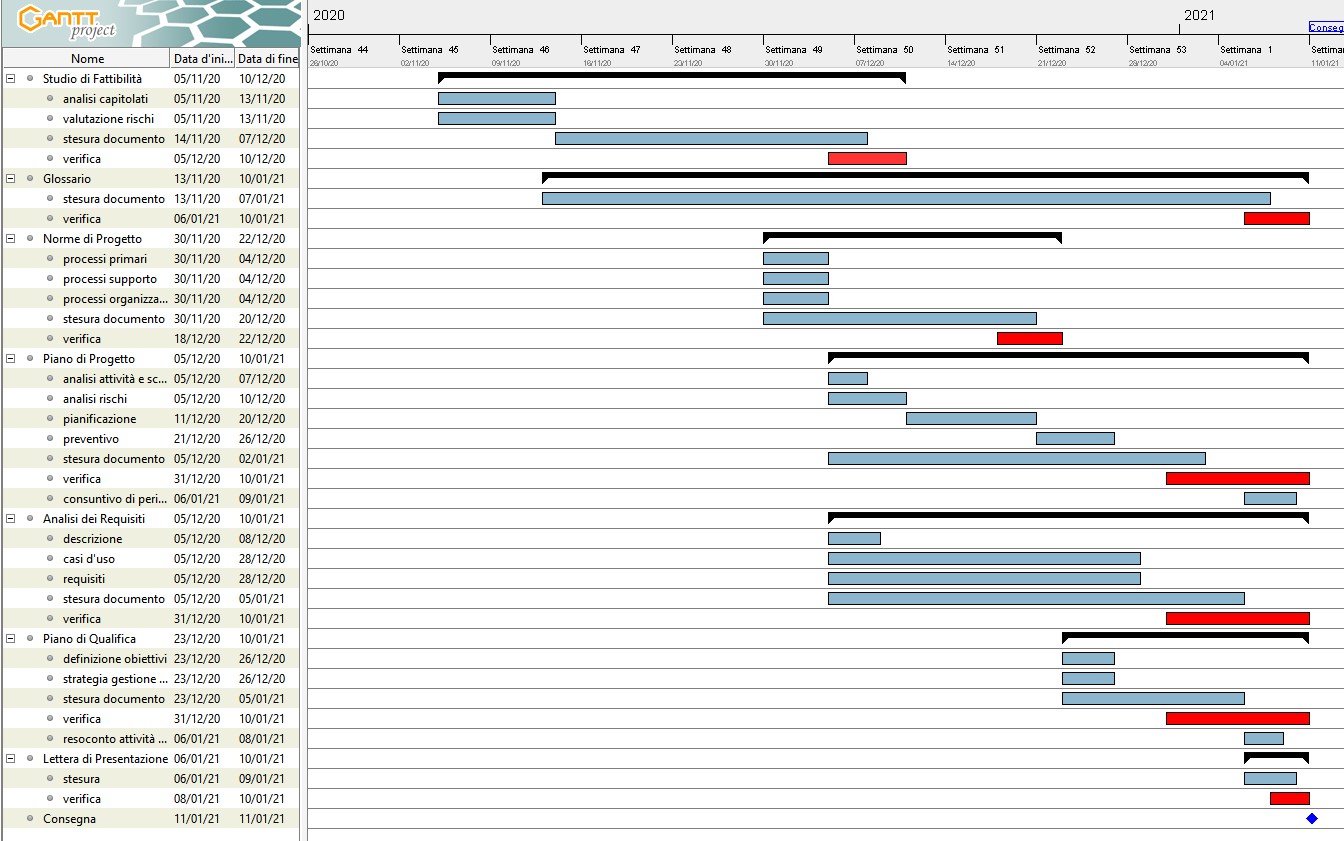
\includegraphics[scale=0.45]{Images/GanttPianificazioneAnalisi.PNG}
	\caption{Diagramma di Gantt dell'attività di Progettazione di dettaglio e Codifica}
\end{figure}
